\section{Clustering}
To optain the class labels used in the classification process, the simple k-Means clustering algorithm is applied to the attribute "total number of violent crimes per
100K population". By using the elbow-method to search for the most significant k, k equals three was revealed as the best parameter as shown in \fref{fig:sse}.
\begin{figure}[H]
	\centering
	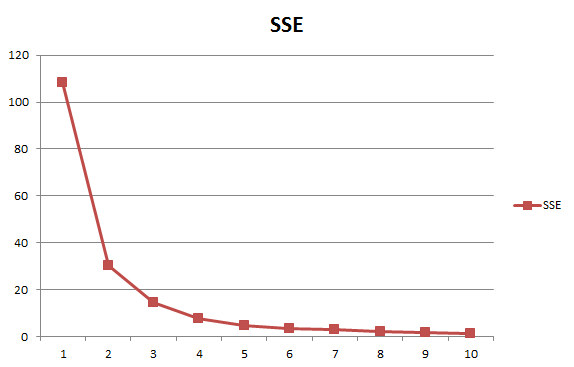
\includegraphics[width=\columnwidth]{../../charts/SSE.png}
	\caption{Sum of the squared errors for different choices of k}
	\label{fig:sse}
\end{figure}
The three classes originating from this choice are namely "High", "Medium" and "Low", the percentage boundaries are respectively:
\begin{description}
	\item[Low:] \([0\%; 22\%]\) 
	\item[Medium:] \((22\%; 56\%]\)
	\item[High:] \((56\%; 100\%]\)
\end{description}

It should be noted, that the authors of \textit{"An Experimental Study of Classification Algorithms for Crime Prediction"} \cite{indian} obtained different results for the percentage boundaries, they did however not disclose the details of their approach. Their percentage boundaries are "Low": \([0\%;25\%)\), "Medium": \([25\%; 40\%)\) and "High": \([40\%; 100\%]\).


